% ==============================================================================
% TCC - Gabriel dos Santos Sereno
% Capítulo 2 - Referencial Teórico
% ==============================================================================
\chapter{Referencial Teórico}
\label{sec-referencial}

Neste capítulo são apresentados os métodos e conceitos necessários para o desenvolvimento do estudo. A seção \ref{subsec-caracteristicas} detalha todos os métodos de seleção de características utilizados no comparativo para a demonstração dos resultados. A seção \ref{subsec-classificador} explica o classificador utilizado no modelo proposto, bem como seu funcionamento interno. Por fim, a seção \ref{subsec-decompondo} faz um comparativo entre duas técnicas populares na literatura de decomposição de problemas multi-classe.

\section{Seleção de Características}
\label{subsec-caracteristicas}

A seleção de características é basicamente formada por um critério de seleção e uma estratégia de busca. Um algoritmo simples seleciona um subconjunto das variáveis que descrevem o processo, preservando apenas as características mais importantes para o modelo, a fim de remover as características supérfluas e maximizar as pontuações de desempenho. O critério de desempenho pode ser a precisão do diagnóstico de falhas. No entanto, em um desequilíbrio extremo entre a disponibilidade de exemplos para o comportamento normal e de falha, métricas alternativas, como $F_{1}$, podem ser mais apropriadas. Considere, por exemplo, um conjunto de dados em que uma em cada 100 amostras é uma falha. Nesse caso, uma precisão de 99\% seria equivalente a um resultado de uma classificação aleatória.

\subsection{Shapley additive explanations (SHAP)}

O SHAP é um método baseado na teoria dos jogos para descrever o desempenho de um modelo de aprendizado de máquina. O principal objetivo dessa técnica é produzir um modelo interpretável e, em seguida, usar as características mais importantes detectadas que contribuíram principalmente para os resultados da classificação, especificamente no diagnóstico de falhas.

No artigo \cite{lundberg2017unified}, o modelo interpretável é definido como $f$ e o modelo de explicação como $g$. O objetivo é explicar o modelo interpretável com uma única entrada $x$. O modelo de explicação usa entradas simplificadas $x'$ para mapear as entradas originais por meio de uma função de mapeamento:

\begin{equation}
  \label{localAccuracyexplanation}
  x = h_{x}(x'),
\end{equation}
onde $h_{x}$ remapeia uma entrada simplificada para a entrada original, em outras palavras, converte um vetor binário de entradas interpretáveis para o espaço de entrada original. Portanto, a função de mapeamento tenta garantir que
\[
  g(z') \approx f(h_{x}(z'))
\]
sempre que,
\[
  z' \approx x',
\]
onde $z'$ é um subconjunto das entradas não nulas $x'$.

Além disso, o algoritmo se concentra em três princípios: precisão local, ausência de informações e consistência. A precisão local é a propriedade de aproximar o modelo original $f$ para uma entrada específica $x$. Isso requer que o modelo de explicação $g$ corresponda à saída $f(x)$ com a entrada simplificada $x'$, garantindo que essa saída seja a soma das atribuições de características, onde ocorre a multiplicação da entrada simplificada $x'$ com o efeito $\phi$, que ocorre quando a função de mapeamento \ref{localAccuracyexplanation} é usada.

Além disso, o modelo de explicação, sendo uma função linear de variáveis binárias que garante a precisão local, pode ser definido da seguinte forma:
\begin{equation}
  \label{localAccuracy}
  f(x) = g(z') = \phi_{0} + \sum_{i = 1}^{M} \phi_{i}z'_{i},
\end{equation}
onde $z' \in {0, 1}^{M}$ é um vetor binário, com $M$ sendo o número de características da entrada simplificada, e $\phi$ é o efeito para cada característica. Esse efeito é o valor de Shapley, sendo calculado a partir da equação \ref{consistency}, determinando se a característica é relevante ou não. Em seguida, pode ser comprovado que o modelo de explicação $g(x')$ corresponde ao modelo original $f(x)$ quando $x = h_{x}(x')$.

A propriedade de ausência de informações impede que a entrada original não tenha nenhum impacto após uma entrada simplificada com características ausentes ter sido submetida ao modelo. Essa propriedade é alcançada quando
\begin{equation}
  \label{missingness}
  x'_{i} = 0 \Rightarrow  \phi_{i} = 0,
\end{equation}
significando que uma entrada zero específica de uma característica $x_{i}$ não causa nenhum efeito $\phi_{i}$ dessa característica.

Por fim, a consistência é alcançada quando um modelo altera $f'$ de modo que uma entrada simplificada $x'$ não mude ou diminua sua importância, independentemente de outras entradas.
Se
\[
  f_{x}(z') = f(h_{x}(z')).
\]
Então
\[
  z' = 0,\quad f_{x}'(z') - f_{x}'(z' \setminus i) \ge f_{x}(z') - f_{x}(z' \setminus i).
\]
Isso implica para todas as entradas $z' \in {0,1}^{M}$, que
\[
  \phi_{i}(f', x) \ge \phi_{i}(f, x).
\]
A única condição que suporta essa ideia é se:
\begin{equation}
  \label{consistency}
  \phi_{i} = \sum_{z' \subseteq x'}^{}\frac{\left| z' \right|!(M - \left| z' \right| - 1)!}{M!} \left[ f_{x}(z' \cup \{i\}) - f_{x} (z') \right],
\end{equation}
onde $|z'|$ representa o número de entradas não nulas em $z'$, e $z' \subseteq x'$ representa todos os vetores $z'$ com um subconjunto de entradas não nulas $x'$. Portanto, $\phi_{i}$ da equação \ref{consistency} são os valores de Shapley que medem a contribuição marginal de cada característica para o resultado previsto. Essa fórmula é calculada considerando todas as combinações possíveis de características e as diferenças no modelo. Além disso, o SHAP tem várias versões, como Kernel SHAP, Deep SHAP e Tree SHAP, que foram usadas neste artigo em conjunto com o modelo Random Forest.

\subsection{Recursive Feature Elimination (RFE)}

O RFE (Recursive Feature Elimination) é um método de seleção de característica baseado no sistema de ranqueamento de acordo com a importância de cada característica. Essa importância representa a quantificação da contribuição de cada característica para resolução do problema, em outras palavras, o classificador com as características mais importantes, tem grandes chances de determinar corretamente a classe do dado fornecido. O algoritmo inicialmente analisa todas as características e, em seguida, define em ordem decrescente o ranque de cada uma. Em seguida, identifica a característica mais fraca com base em métricas de avaliação do modelo (como $F_{1}$-score) e a remove \cite{granitto2006recursive}. Como esse processo é iterativo, o modelo é ajustado novamente até atingir o número desejado de características a serem selecionadas, definido por hiperparâmetro. O procedimento de remoção iterativa é necessário porque, após a eliminação da característica, a importância de cada característica muda substancialmente, exigindo um recálculo \cite{guyon2002mach}.

\begin{algorithm}
  \caption{Recursive Feature Elimination (RFE)}
  \label{alg:rfe}
  \begin{algorithmic}[1]
    \REQUIRE{Base de dados $\mathcal{D}$ com características $\mathbf{X}$, classificador $\mathcal{C}$, número de características para selecionar $k$}
    \ENSURE{Características selecionadas $\mathbf{X}_{\text{selecionado}}$}
    \STATE Inicializar $\mathbf{X}_{\text{selecionado}} \leftarrow \mathbf{X}$
    \WHILE{Número de características em $\mathbf{X}_{\text{selecionado}}$ é maior que $k$}
    \STATE Treinar $\mathcal{C}$ com $\mathbf{X}_{\text{selecionado}}$
    \STATE Computar as importâncias da características utilizando $\mathcal{C}$
    \STATE Identificar a característica com a menor importância e remove-la de $\mathbf{X}_{\text{selecionado}}$
    \ENDWHILE
    \RETURN $\mathbf{X}_{\text{selecionado}}$
  \end{algorithmic}
\end{algorithm}

As importâncias de cada característica podem ser calculadas de diversas formas, como por coeficientes, pesos e permutação. Os coeficientes são principalmente utilizados em modelos lineares, como no estudo de \cite{fonti2017feature}, já que esses coeficientes recebem uma característica para quantificar a mudança na variável alvo. Com isso, características que afetam fortemente essa variável tende a serem classificadas como mais importantes. Já na utilização de pesos, são unicamente utilizados em modelos de árvores, onde maiores pesos determinam características que dividem melhor os dados para classificar nos nós das árvores, como utilizado no estudo \cite{zhou2021landslide}. E por fim a permutação, introduzido inicialmente por \cite{breiman2001random}, pode ser utilizado em diversos modelos, na qual consiste em modificar a ordem de apenas uma característica, deixando as demais estáticas. Caso o algoritmo identifique que o desempenho diminuiu drasticamente a partir de métricas como a acurácia, o RFE determina que essa característica é de suma importância para o modelo.

Por fim, o RFE como método de seleção de características tem como beneficio a simplicidade e também a rapidez na seleção. Ideal para problemas que não requerem uma seleção de caraterísticas tão complexas e que exigem performances melhores em troca do uso computacional e tempo. Além disso, o método é de simples interpretação, onde o utilizador consegue entender porque tal característica não influencia no atual problema proposto \cite{chen2007enhanced}. Outro benefício do RFE pode ser utilizado por vários classificadores e dependendo do classificador escolhido, o resultado das características selecionadas pode se tornar diferente.

Portanto, devido ao bom desempenho nos estudos feitos por diversos autores como: \cite{shao2017new} que utilizou o método para selecionar melhores características na predição de valores a serem pagos em contas de energia, já \cite{richhariya2020diagnosis} que utilizou para selecionar melhores características no diagnóstico de Alzheimer e \cite{zhou2021landslide} que utilizou para selecionar melhores características no mapeamento de suscetibilidade, o RFE foi usado na comparação com o SHAP proposto neste estudo.

\subsection{Selection from Model (SFM)}

O Selection from Model é um algoritmo básico de seleção de características baseado em modelo criado pelos autores. Para isso, para cada característica foi atribuído uma importância de acordo com o modelo. Por exemplo, a importância de cada característica utilizando o modelo Random Forest são representados pelo ganho de informação, mais especificamente pelo ganho de impureza do índice de Gini de cada característica \cite{breiman1984classification}. Dessa forma, com a atribuição dessa importância para cada característica, é feito o ranqueamento e seleção das N primeiras características para compor o novo conjunto de dados.

O principal benefício desse algoritmo é a sua simplicidade, por apenas utilizar os N primeiras características mais importantes, não requer quase nenhum poder computacional. Entretanto, a eficiência do método é ser comprometida por não haver nenhum parâmetro no momento da seleção, apenas o número máximo de características informado pelo usuário.

Foi introduzido esse algoritmo como base no comparativo, permitindo a comparação da força entre um algoritmo que emprega cálculos e métodos na seleção.

\subsection{Mutual Information (MI)}

O Mutual Information foi descrito por \cite{vergara2014vergara} como um poderoso método de seleção de características que possui duas propriedades principais. Em primeiro lugar, qualquer tipo de relação entre variáveis aleatórias pode ser medida. Em segundo lugar, o Mutual Information preserva a ordem dos elementos originais, mesmo após a aplicação de uma transformação, como rotações ou translações de dados.

O Mutual Information estima a informação mútua entre duas características aleatórias, onde valores mais altos indicam uma dependência maior e um valor aproximadamente zero indica uma dependência menor. O método é baseado na estimativa de entropia a partir da distância dos k-vizinhos mais próximos, que foi originalmente proposto por \cite{kraskov2011erratum}. Este método foi escolhido para ser comparado devido à quantificação da importância entre duas características aleatórias, o que pode resultar em resultados significativamente diferentes.

Os benefícios na utilização desse método de seleção de variáveis são focados na principal característica do Mutual Information, a análise da correlação entre os dados. O método consegue capturar relacionamentos não-lineares, tornando possível a identificação de dependências complexas que não são detectadas por métodos lineares. Além disso, é mais suscetível que o método selecione características é melhor em conjunto com outras características do que a característica individualmente. Por fim, o Mutual Information pode ser aplicado na grande maioria dos domínios, como classificação, regressão e clustering sem grandes modificações no método e nem no dado de entrada \cite{bao2008evaluation}.

Entretanto, o método por ser poderoso ao estimar os relacionamentos através de cálculos matemáticos pode ser computacionalmente custoso com base de dados grandes ou com alta dimensionalidade. Esse problema é explorado neste estudo cientifico \cite{shams2007speeding}, onde é utilizado NVIDIA CUDA para aprimorar o desempenho do algoritmo. Ademais, por focar extremamente na correlação dos dados, a seleção de características pode ser comprometida, pois o algoritmo não consegue definir se essa combinação é relevante ou não para o problema proposto. Por fim, o Mutual Information é limitado a verificar a correlação entre duas variáveis, não sendo possível identificar um conjunto maior que contem mais interações \cite{bao2008evaluation}.

Portanto, além de entender os pontos fortes e fracos do método, foi verificado estudos reais que utilizaram Mutual Information como um método de seleção de características. Como por exemplo, o estudo de \cite{amiri2011mutual} que utiliza o método integrando um modelo com o objetivo de detectar intrusões em sistemas. Além desse estudo, \cite{verron2008fault} utiliza o Mutual Information justamente no mesmo principio deste estudo, a detecção e identificação de falhas no processo químico Tennessee Eastman. E por fim, a utilização do método em diagnósticos assistidos por computador \cite{tourassi2001application}.

\subsection{ANOVA F-Value}

De acordo com \cite{doan2020designing}, o \textit{ANOVA F-Value} é uma análise estatística que seleciona características com base na dependência de cada característica usando as estatísticas F. Essa dependência pode ser determinada calculando a variação em termos de categorias em relação às variações individuais. Uma abordagem sólida para remover características que não possuem importância é calcular a significância estatística, onde $p\text{-value} < 0.05$ ou $p\text{-value} < 0.01$, conforme relatado por \cite{campbell2018differentially}.

Os benefícios de utilizar esse método são intrinsecamente relacionados ao cálculo do $p\text{-value}$ entre características, na qual determina se a característica será retirada ou não dependendo da sua significância estatística. Com isso, o ANOVA F-Value possui boa interpretabilidade, pois a partir das características em que o método determinou como significante, é possível concluir a razão da seleção para um determinado caso.

Embora o ANOVA F-Value tenha importantes qualidades, o método requer que os dados estejam normalmente distribuídos e que a variação dentre os grupos sejam homogêneas e categóricos. Ao contrário do método Mutual Information, o ANOVA F-Value não considera potenciais relações entre as características, podendo remover importantes características que em conjunto, poderiam demonstrar melhor a classe correta.

O \textit{ANOVA F-Value} foi escolhido para compor o comparativo pela sua relevância entre os estudos científicos como \cite{ding2014identification} que utilizou o método na identificação de proteínas de bacteriófagos. Além desse estudo, \cite{elssied2014novel} utilizou o \textit{ANOVA F-Value} como método de seleção de características para auxiliar na classificação de spam de e-mails. Por fim, \cite{sheikhan2013modular} que utilizou o método para selecionar as melhores características para detectar a emoção através da voz. Portanto, o \textit{ANOVA F-Value} é largamente utilizado no meio acadêmico e cientifico, além de ser reconhecido como um método eficaz para seleção de características.

\section{Classificador}
\label{subsec-classificador}

Em aprendizado de maquinas, um classificador é um algoritmo que recebe dados de entrada e o determina como uma dentre várias classes baseado no relacionamento dos dados de treinamento, na qual foram separados antes da execução do algoritmo. O principal objetivo de um classificador é identificar a classe de um dado nunca utilizado anteriormente e o classificando através da generalização vinda do padrão aprendido durante a fase de treinamento \cite{pereira2009machine}.
Nesse sentido, o classificador possui quatro fases (Figura \ref{fig-workflow}) até a predição da classe \cite{mohammed2016machine}:

\begin{itemize}
  \item Treinamento: Durante essa fase, é introduzido ao classificador uma base de dados que contém rótulos. Como por exemplo, um classificador que tem como objetivo identificar números escritos a mão, esses dados provavelmente serão o valor do pixel de uma imagem junto a um rótulo, que nesse caso será um número.
  \item Aprendizado de Padrões: Com a informação recebida dos dados de treinamento, o classificador utiliza diversas técnicas e fórmulas matemáticas para identificar padrões através do relacionamento entre os dados. Por exemplo, um classificador pode identificar os padrões do número 1, que pode ser escrito de diferentes formas por diversas pessoas, mas é reconhecível porque há um padrão na escrita desse número. Ao aprender com esses padrões durante a fase de treinamento, o classificador se torna capaz de generalizar e classificar corretamente novos dados nunca antes vistos.
  \item Teste: Depois do classificador treinado, é introduzido ao classificador uma base de dados de testes que não contém rótulos. Esses dados introduzidos nunca foram vistos pelo classificador durante o treinamento. Neste momento, é calculado principalmente a acurácia e outras métricas importantes na intenção de verificar quão correto o classificador avaliou os novos dados.
  \item Predição: Após todas essas etapas e ajustes no classificador, o classificador estará pronto para o funcionamento, identificando novos dados e rotulando-os de acordo com o padrão analisado.
\end{itemize}

\begin{figure}
  \centering
  \begin{tikzpicture}[node distance=2cm, auto]
    \node (database) {Banco de Dados};
    \node [below left of=database] (traindata) {Dados de Treinamento};
    \node [below right=.85cm and 0cm of database] (testdata) {Dados de Teste};
    \node [below of=traindata] (train) {Aprendizado de Padrões};
    \node [below of=train] (test) {Testes};
    \node [below of=test] (predict) {Predição};

    \path[->] (database) edge (traindata);
    \path[->] (database) edge (testdata);
    \path[->] (traindata) edge (train);
    \path[->] (train) edge (test);
    \path[->] (testdata) edge[bend left] (test);
    \path[->] (test) edge (predict);
  \end{tikzpicture}
  \caption{Fases do classificador}
  \label{fig-workflow}
\end{figure}

Então, com um classificador é possível utilizar para diversas finalidades, como o estudo de \cite{pal2005random} que utiliza classificadores para identificar em uma determinada área da zona rural, quais são os tipos de plantação através de imagens. Além disso, o estudo \cite{zhang2018hybrid} utiliza classificadores que são modelos de Deep Learning para identificar a quantidade de objetos presente no ambiente em imagens, como árvores, construções, rios. E também para a finalidade de detectar e identificar falhas como nos trabalhos de \cite{wang2016wind}, \cite{neupane2020bearing} e \cite{saufi2019challenges}. Isso é apenas possível pois o classificador identifica padrões e a relação entre os dados.

Há diversos tipos de classificadores e neles incluem \cite{ayodele2010types}:

\begin{itemize}
  \item Regressão Linear: Utiliza a matemática da regressão linear para classificação binária através de uma reta trassada entre os dados e separando-os.
  \item Arvore de Decisão: Estruturas em formato de árvore que utiliza sequencia binária de decisões para classificar tanto problemas multi-classe tanto binário.
  \item Random Forest: Um conjunto de Arvores de Decisão, na qual utiliza o resultado da maioria das arvores como a classificação final.
  \item Naive Bayes: Baseado no teorema de Bayes e comumente utilizado para classificação de textos.
  \item Neural Networks: São modelos de Deep Learning em que lidam com padrões de dados complexos e em grande quantidade.
\end{itemize}

A escolha de um classificador depende de vários fatores, como a natureza do problema, a quantidade de dados disponível, o nível de interpretabilidade, o tempo de treinamento e demais fatores. Cada classificador possui pontos fortes e fracos, então é essencial o experimento e a escolha apropriada para a tarefa a ser resolvida \cite{ray2019quick}.

Nesse trabalho, é necessário o uso de métodos de seleção de características que se baseiam no classificador. Por isso, o classificador Random Forest foi o mais apropriado, já que a partir dos dados coletados, o classificador se ajusta para escolher as melhores características para diagnosticar a classe do dado, além de ter a vantagem do modelo ser de fácil interpretação. Para o entendimento desse comportamento, a próxima subseção irá entrar em detalhes como o algoritmo de Random Forest opera.

O Random Forest é um classificador formado por um conjunto de árvores de decisão. Para o entendimento profundo do classificador Random Forest, precisamos entender primeiro as árvores de decisão. Uma árvore de decisão é um grafo acíclico direcionado em que cada nó é divido por seus sucessores, podendo uma delas ser uma nó folha ou nó de divisão \cite{myles2004introduction}, como mostra na Figura \ref{fig-decisiontree}.

\begin{figure}
  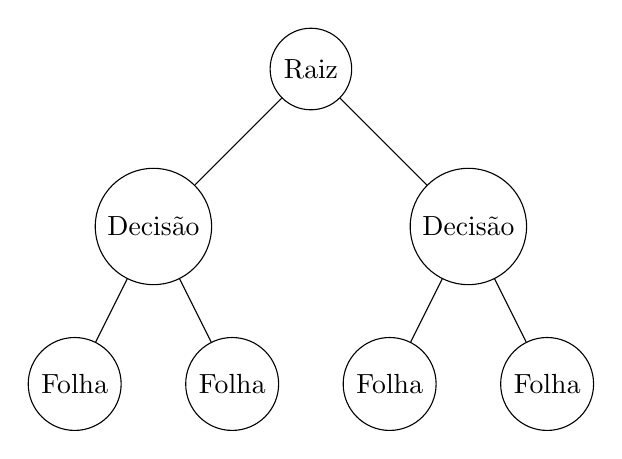
\begin{tikzpicture}[
      every node/.style={circle, draw},
      level 1/.style={sibling distance=4cm},
      level 2/.style={sibling distance=2cm},
      level distance=2cm
    ]

    \node {Raiz}
    child {
        node {Decisão}
        child {
            node {Folha}
          }
        child {
            node {Folha}
          }
      }
    child {
        node {Decisão}
        child {
            node {Folha}
          }
        child {
            node {Folha}
          }
      };

  \end{tikzpicture}
  \centering
  \caption{A árvore de decisão e sua estrutura.}
  \label{fig-decisiontree}
\end{figure}

O nó de uma árvore de decisão, é o ponto onde contem um teste condicional, na qual determina os seus sucessores.
Dessa forma, as árvores de decisão são fáceis de interpretar e visualizar. Além de poder classificar tanto dados categóricos e numéricos. Entretanto, as árvores de decisão podem sofrer com overfitting, especialmente quando é criado diversos nós, criando mais complexidade na árvore, pois os nós contem testes condicionais muito específicos, perdendo o atributo de generalização e portanto a taxa de acurácia. Uma forma de prevenir esse problema é efetuar a técnica de poda, onde propositalmente é removido esses nós para a árvore ser mais genérica.

\begin{figure}
  \begin{forest}
    for tree={edge={-latex},l=2cm}
    [Todos os dados, rectangle, draw
      [Raiz 1, circle, draw, edge label={node[midway,left,font=\scriptsize]{Conjunto Aleat.}}
          [Variável 1, edge label={node[midway,left,font=\scriptsize]{Sim}}
              [Folha 1, edge label={node[midway,left,font=\scriptsize]{Sim}}]
              [Folha 2, edge label={node[midway,right,font=\scriptsize]{Não}}]
          ]
          [Variável 2, edge label={node[midway,right,font=\scriptsize]{Não}}
              [Folha 3, edge label={node[midway,left,font=\scriptsize]{Sim}}]
              [Folha 4, edge label={node[midway,right,font=\scriptsize]{Não}}]
          ]
      ]
      [Raiz 2, circle, draw, edge label={node[midway,right,font=\scriptsize]{Conjunto Aleat.}}
          [Variável 3, edge label={node[midway,left,font=\scriptsize]{Sim}}
              [Folha 5, edge label={node[midway,left,font=\scriptsize]{Sim}}]
              [Folha 6, edge label={node[midway,right,font=\scriptsize]{Não}}]
          ]
          [Variável 4, edge label={node[midway,right,font=\scriptsize]{Não}}
              [Folha 7, edge label={node[midway,left,font=\scriptsize]{Sim}}]
              [Folha 8, edge label={node[midway,right,font=\scriptsize]{Não}}]
          ]
      ]
    ]
  \end{forest}
  \centering
  \caption{O Random Forest e sua estrutura}
  \label{fig-randomforest}
\end{figure}

Como mostra na Figura \ref{fig-randomforest}, o Random Forest é um conjunto de árvores de decisão. Cada árvore é treinado com uma porção aleatória dos dados e a predição dessas árvores são unidas para a decisão final.

O algoritmo Random Forest é altamente eficiente na identificação das complexidades presentes nos dados, permitindo que as árvores de decisão possuam uma maior capacidade de generalização. Ao contrário de uma única árvore de decisão que abrange todas as características, o Random Forest subdivide essas características entre várias árvores, permitindo que cada uma delas explique melhor as relações presentes nos dados.

Uma das principais vantagens do Random Forest é a melhora significativa na classificação dos dados. Isso é alcançado por meio da combinação das decisões de todas as árvores em um processo de votação, onde a classe mais frequente é selecionada como o resultado final. Essa abordagem coletiva garante uma maior robustez e precisão no processo de classificação, tornando o algoritmo uma poderosa ferramenta para diversas tarefas de aprendizado de máquina \cite{breiman2001random}.

\section{Decompondo conjuntos de dados multiclasse}
\label{subsec-decompondo}

Em Aprendizado de Máquina, diversos cenários são extremamente complexos e que requer um ótimo
classificador para identificar diversas classes de um banco de dados. Para isso, existe a técnica
de decomposição, na qual particiona o problema em pequenas partes.

Em classificação multi-classe, a estratégia de decomposição é uma valiosa ferramenta para habilitar
o uso de classificadores binários em situações onde anteriormente não eram viáveis devido
à complexidade do problema. Com essa abordagem, torna-se possível testar múltiplos
classificadores binários e verificar se algum deles contribui de forma mais eficaz para
a identificação das diferentes classes \cite{elkano2016fuzzy}.

Para lidar com essa limitação, existem dois tipos de métodos de decomposição que transformam
problemas multi-classe em subproblemas binários, são eles One-vs-All (OVA) e One-vs-One (OVO).
Para a escolha, é necessário entender os fatores em que uma técnica tem maiores benefícios que
a outra, pois dependendo do número de classes, características da base de dados e recurso computacional,
uma de ambas as técnicas pode sobressair e ter melhores resultados \cite{li2020multiclass}.

% \begin{center}
%   \textbf{Classificadores} \\
%   \( \hat{f}_1 \quad \hat{f}_2 \quad \hat{f}_3 \quad \hat{f}_4 \) \\
%   \begin{tikzpicture}
%     \matrix (m) [matrix of math nodes,row sep=3em,column sep=4em,minimum width=2em]
%     {
%       +1 & -1 & -1 & -1 \\
%       -1 & +1 & -1 & -  \\
%       -  & -  & +  & +  \\
%       +  & +  &    &    \\
%     };
%   \end{tikzpicture} \\
%   (4) \times (1,2,3) \\
%   (3) \times (1,2,4) \\
%   (2) \times (1,3,4) \\
%   (1) \times (2,3,4)
% \end{center}

\subsection{One-vs-All (OVA)}

Em OVA, para N classes, N classificadores binários são treinados, sendo que cada um tem como objetivo
distintivo identificar uma classe específica em relação a todas as outras agrupadas. Por exemplo,
dado um classificador binário especializado na classe A é treinado para identificar
apenas dados da classe A como positiva e todas as demais negativas \cite{zhang2019multi}.
Portanto, durante a predição dos dados, cada classificador gera a probabilidade exclusiva de sua
classe, e, dessa forma, é verificado qual classe corresponde a uma determinada entrada com base
no maior score obtido entre os classificadores.

\subsection{One-vs-One (OVO)}

Em OVO, para N classes, N(N-1)/2 classificadores binários são treinados, sendo que cada um
tem como objetivo distintivo identificar uma classe específica em relação a outra. Por
exemplo, durante o treinamento, um classificador binário especializado na classe A recebe
como entrada a classe A e a classe B para serem treinados e identificar apenas a classe
A como positiva e a classe B como negativa \cite{pawara2020one}. Portanto, durante a predição
dos dados, cada classificador faz sua própria decisão, e a classe com o maior voto dentre os
classificadores é escolhido para ser a predição final.